\documentclass[12pt]{beamer}
\usetheme{Pittsburgh}
\usepackage[T1,T2A]{fontenc}
\usepackage[utf8]{inputenc}
\usepackage[bulgarian]{babel}
%\usepackage{amsmath}
%\usepackage{amsfonts}
%\usepackage{amssymb}
\usepackage{graphicx}

%\usepackage{enumerate}
%\usepackage{soul}


\title{Информационна система на агенция за недвижими имоти}
\subtitle{Част II: Модел на потребителските случаи}
\author{Екип $\pi \approx 3.1$}

%\setbeamercovered{transparent} 
\setbeamertemplate{navigation symbols}{} 
\date{} 

\begin{document}

\begin{frame}
\titlepage
\end{frame}

%\begin{frame}
%\tableofcontents
%\end{frame}

\begin{frame}[fragile]
\frametitle{Модел (А)}
        \begin{figure}[h]
        \centering
        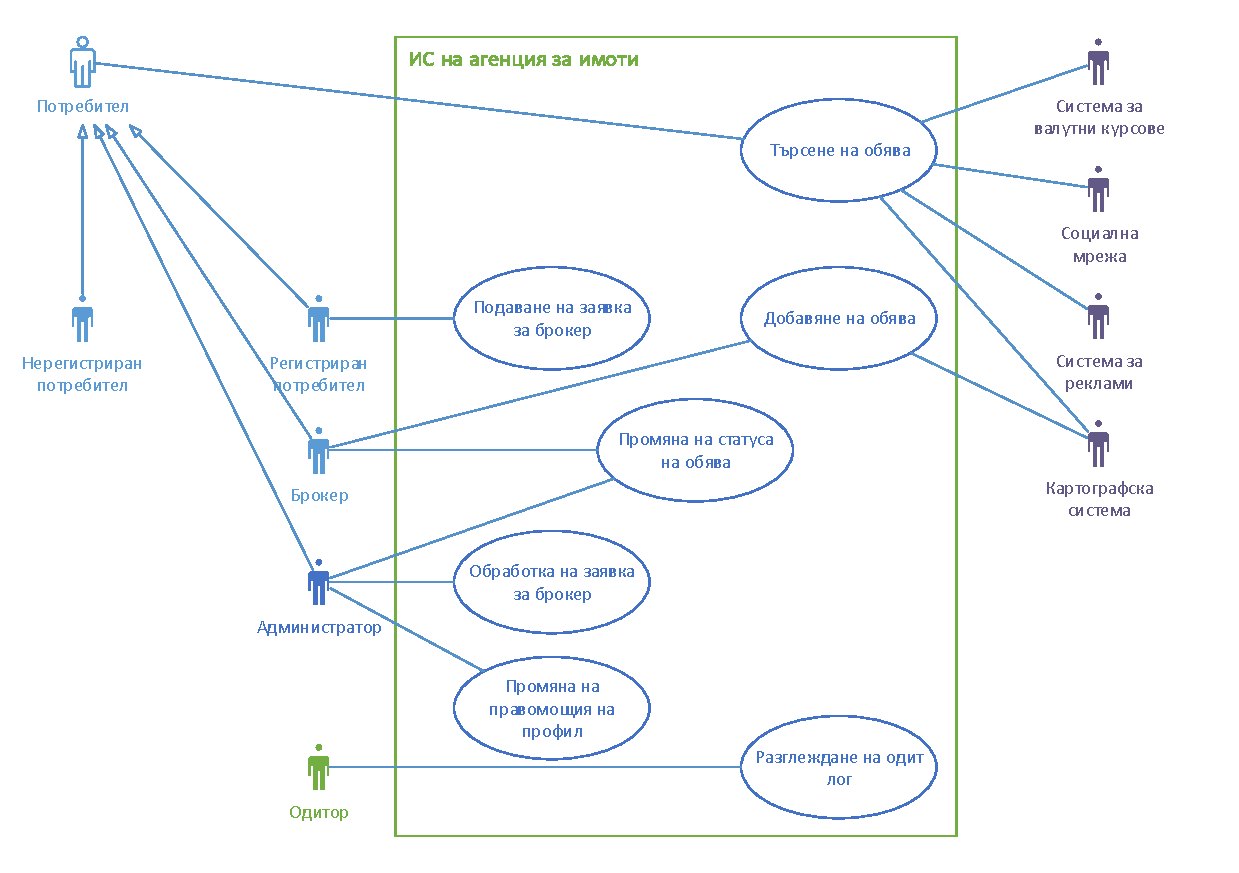
\includegraphics[scale=0.5]{uc1-a}
%        \caption{Use case модел на потребителските случаи с приоритет A}
        \end{figure}
\end{frame}

\begin{frame}[fragile]
\frametitle{Модел (B)}
        \begin{figure}[h]
        \centering
        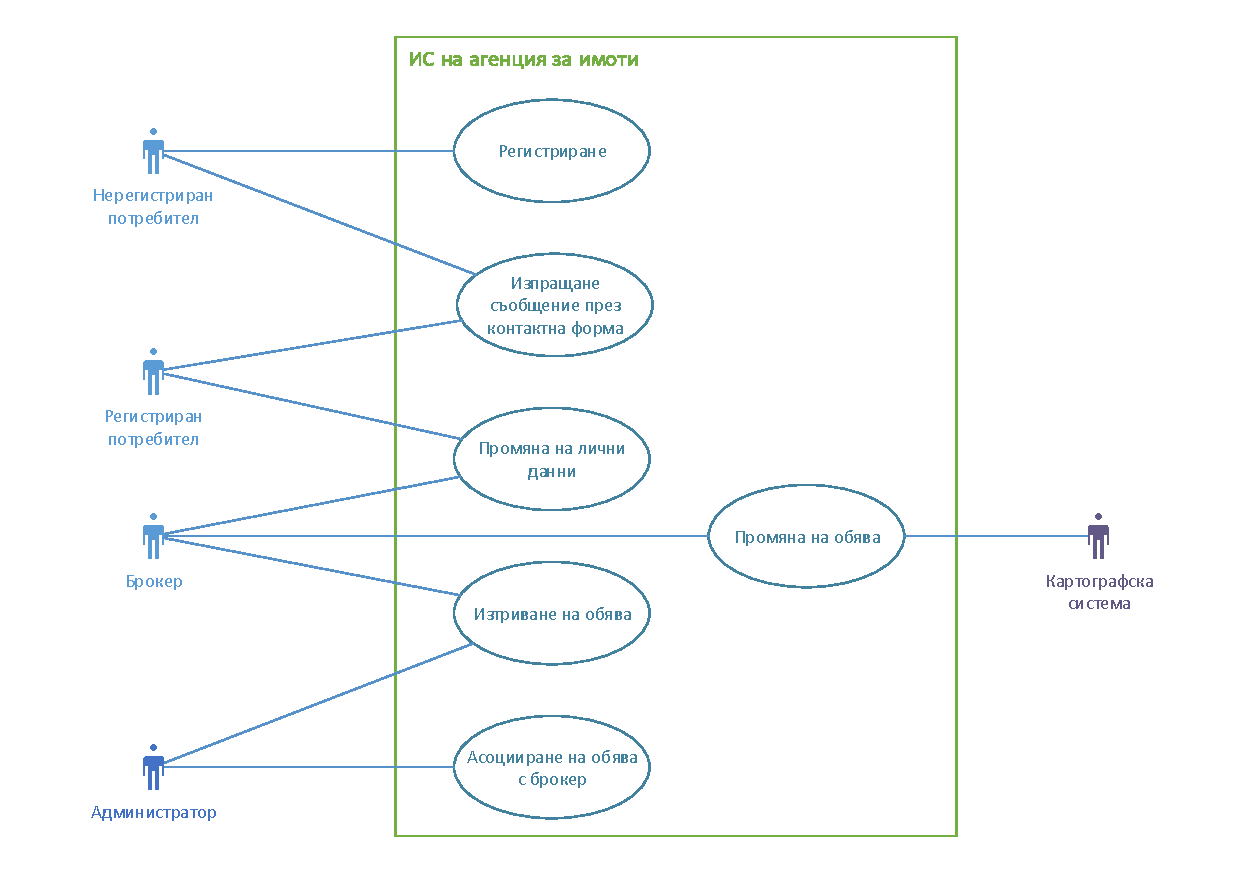
\includegraphics[scale=0.5]{uc1-b}
%        \caption{Use case модел на потребителските случаи с приоритет A}
        \end{figure}
\end{frame}

\begin{frame}[fragile]
\frametitle{Модел (C)}
        \begin{figure}[h]
        \centering
        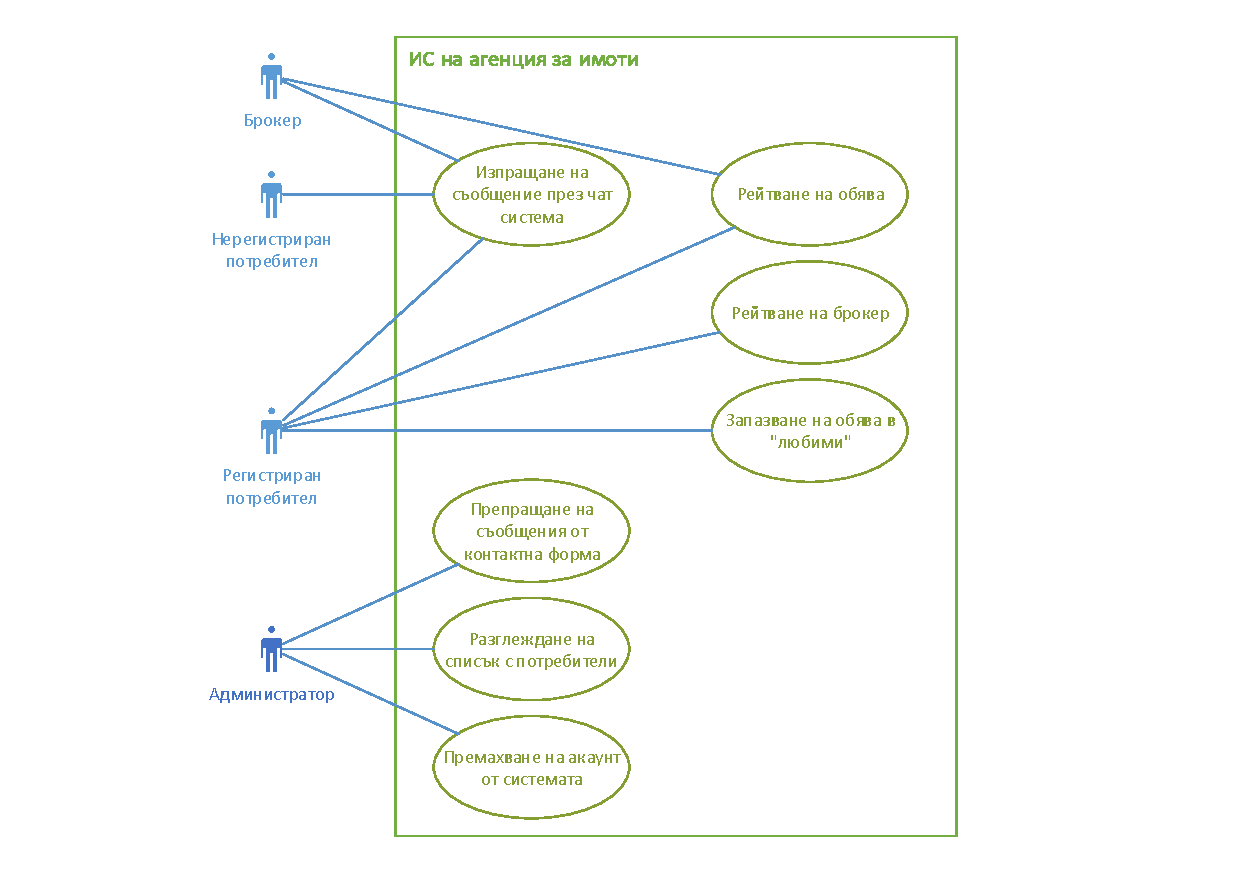
\includegraphics[scale=0.5]{uc1-c}
%        \caption{Use case модел на потребителските случаи с приоритет A}
        \end{figure}
\end{frame}

\begin{frame}[fragile]
\frametitle{Use case template (1)}
\begin{itemize}
	\item Use Case \textit{<номер>} \textit{<име на потребителският случай>}
	\item Level: \textit{<user-goal или subfunction>}
	\item Primary Actor: \textit{<основен актьор>}
	\item Stakeholders: \textit{<списък на заинтересовани лица и техните интереси>}
	\item Preconditions: \textit{<предусловия>}
	\item Postconditions: \textit{<следусловия>}	
	\item Trigger: \textit{<стартиране>}
\end{itemize}
\end{frame}

\begin{frame}[fragile]
\frametitle{Use case template (2)}
\begin{itemize}
	\item {Main Success Scenario:
		\begin{enumerate}
			\item \textit{<стъпка>}
			\item \textit{<стъпка>}
		\end{enumerate}
	}
	\item {Extensions:
		\begin{itemize}
			\item[2.a] {\textit{<Алтернативна стъпка на такава от основния сценарий>}
				\begin{enumerate}
					\item[1.] \textit{<стъпка от алтернативния сценарий>}
					\item[2.] \textit{<стъпка от алтернативния сценарий>}                
				\end{enumerate}
			}
			\item[5.a] {\textit{<Алтернативна стъпка на такава от основния сценарий>}
				\begin{enumerate}
					\item[1.] \textit{<стъпка от алтернативния сценарий>}
					\item[2.] \textit{<стъпка от алтернативния сценарий>}                
				\end{enumerate}
			}
		\end{itemize}
	}                
\end{itemize}
\end{frame}

\begin{frame}[fragile]
\frametitle{Use case template (3)}
\begin{itemize}
	\item Special Requirements: \textit{<специални изисквания>}
	\item Frequency of Occurrence: \textit{<колко често се случва потребителският случай>}
	\item Notes: \textit{<Незадължително поле за коментари и въпроси>}
\end{itemize}
\end{frame}

\begin{frame}[fragile]
\frametitle{Добавяне на обява (1)}
\begin{itemize}
	\item Use Case: A-2 Добавяне на обява
	\item Level: user-goal
	\item Primary Actor: Брокер
	\item {Stakeholders:
		\begin{itemize}
			\item Брокер: Желае да добави обява в системата.
			\item Купувачи: Желаят да имат обяви в системата, за да имат голям избор, когато търсят и да могат по-лесно да си изберат точния имот за тях.
			\item Продавачи: Желаят възможно най-бързо да продават имота си.
			\item Администратор: Желае в системата да има голям избор от обяви.	
		\end{itemize}
	}
	\item Preconditions: Потребителят е в системата като Брокер
	\item Postconditions: Създава се обява със статус Активна
	\item Trigger: Потребителят избира достъп до функционалност ``Добавяне на обява''
\end{itemize}
\end{frame}

\begin{frame}[fragile]
\frametitle{Добавяне на обява (2)}
\begin{itemize}
	\item {Main Success Scenario:
		\begin{enumerate}
	\item Системата показва полетата, които трябва да се попълнат
	\item Брокерът попълва полетата
	\item Системата проверява данните, въведени от потребителя
	\item Брокерът потвърждава създаването на обявата
	\item Системата създава обявата
	\item Системата обновява статуса на обявата
	\item Системата записва събитието в одит лога
		\end{enumerate}
	}
\end{itemize}
\end{frame}

\begin{frame}[fragile]
\frametitle{Добавяне на обява (3)}
\begin{itemize}
	\item {Extensions:
		\begin{itemize}
        \item[3.a] {Невалидни данни
                \begin{enumerate}[1.]
                \item Системата препраща Брокера към полето с невалидните днани
                \item Системата извежда информативно съобщение относно невалидността на полето
                \item Системата препраща потребителя към стъпка 2 от основния сценарий
                \end{enumerate}
        }
        \item[4.a] {Брокерът не потвърждава създаването на обявата
                \begin{enumerate}[1.]
                \item Системата не създава обявата
                \end{enumerate}
        }
		\end{itemize}
	}                
	\item Special Requirements: N/A
	\item Frequency of Occurrence: Около 70-80 обяви на месец
\end{itemize}
\end{frame}

\begin{frame}[fragile]
\frametitle{Търсене на обява (1)}
\begin{itemize}
	\item Use Case: A-1 Търсене на обява
	\item Level: user-goal
	\item {Primary Actor:
		\begin{itemize}
			\item нерегистриран потребител
			\item регистриран потребител
			\item брокер
			\item администратор
		\end{itemize}
	}
	\item {Stakeholders:
		\begin{itemize}
			\item Потребител: Иска да намери най-подходящата обява за себе си
			\item Брокер: Желае системата да предоставя най-точноотговарящите на потребителските изисквания обяви, както и да сключи сделка с потребителя в най-кратък срок
		\end{itemize}
	}
\end{itemize}
\end{frame}

\begin{frame}[fragile]
\frametitle{Търсене на обява (2)}
\begin{itemize}
	\item Preconditions: N/A
	\item Postconditions: Инициаторът на търсенето е намерил подходящата за себе си обява.
	\item Trigger: Потребителят е влязъл в системата за търсене.
\end{itemize}
\end{frame}

\begin{frame}[fragile]
\frametitle{Търсене на обява (3)}
\begin{itemize}
	\item {Main Success Scenario:
		\begin{enumerate}
      \item Системата предоставя карта на населените места в страната
      \item Потребителят избира населено място от картата
      \item Системата предоставя карта на районите/кварталите в съответното населено място
      \item Потребителят избира район или квартал от предоставената карта
      \item Системата предоставя списък от допълнителни характеризиращи полета към обявата
      \item Потребителят избира желаните от него критерии
		\end{enumerate}
	}	
\end{itemize}
\end{frame}

\begin{frame}[fragile]
\frametitle{Търсене на обява (4)}
\begin{itemize}
  \item {Main Success Scenario (cont.):
    \begin{enumerate}
      \setcounter{enumi}{6}
      \item Потребителят въвежда ключови думи в полето за търсене по свободен текст
			\item Потребителят инициира търсенето
			\item Системата обработва заявката за търсене
			\item Системата предоставя множество от обяви, отговарящи на зададените изисквания
			\item Потребителят разглежда списъка от обяви
			\item Потребителят избира конкретна обява
			\item Потребителят приключва с търсенето
    \end{enumerate}
  }
\end{itemize}
\end{frame}

\begin{frame}[fragile]
\frametitle{Търсене на обява (5)}
\begin{itemize}
	\item {Extensions:
		\begin{itemize}
        \item[1.a] {Потребителят разглежда системата от мобилно устройство
                \begin{enumerate}[1.]
                \item Системата предоставя списък от населените места, вместо карта
                \item Потребителят избира населено място от предоставения списък
                \item Системата предоставя списък от районите/кварталите в избраното населено място
                \item Потребителят избира район или квартал от предоставения списък
                \item Системата препраща потребителя към стъпка 5 от основния сценарий
                \end{enumerate}
        }
		\end{itemize}
	} 
\end{itemize}
\end{frame}

\begin{frame}[fragile]
\frametitle{Търсене на обява (6)}
\begin{itemize}
	\item {Extensions:
		\begin{itemize}
        \item[3.a] {Липсват райони/квартали за избраното населено място
                \begin{enumerate}[1.]
                \item Системата препраща потребителя към стъпка 5 от основния сценарий
                \end{enumerate}
		}
        \item[7.a] {Потребителят не въвежда ключови думи в полето за търсене
                \begin{enumerate}[1.]
                \item Системата препраща потребителя към стъпка 8 от основния сценарий
                \end{enumerate}
        }
		\end{itemize}
	} 
\end{itemize}
\end{frame}

\begin{frame}[fragile]
\frametitle{Търсене на обява (7)}
\begin{itemize}
	\item {Extensions:
		\begin{itemize}
        \item[11.a] {Резултатното множество е празно, т.е. няма обяви отговарящи на зададените критерии
                \begin{enumerate}[1.]
                \item Потребителят променя зададените критерии
                \item Потребителят инициира ново търсене
                \item Системата препраща потребителя към стъпка 9 от основния сценарий
                \end{enumerate}
        }
        \item[11.b] {В резултатното множество липсват обяви, които отговарят на потребителските изисквания
                \begin{enumerate}[1.]
                \item Потребителят променя зададените критерии на търсене
                \item Системата препраща потребителя към стъпка 9 от основния сценарий
                \end{enumerate}
		}
        \item[13.а] {Потребителят се връща към списъка с обяви
                \begin{enumerate}[1.]
                \item Системата препраща потребителя към стъпка 10 от основния сценарий
                \end{enumerate}        
        }
		\end{itemize}
	} 
\end{itemize}
\end{frame}

\begin{frame}[fragile]
\frametitle{Търсене на обява (8)}
\begin{itemize}
	\item {Special Requirements:
		\begin{itemize}
	        \item системата отговаря на заявеното търсене за по-малко от 3 секунди
	        \item обявите с VIP статус се визуализират с приоритет от системата (преди нормалните обяви)
   		\end{itemize}
   	}
	\item Frequency of Occurrence: Много често -- една от най-използваните функционалности в системата
\end{itemize}
\end{frame}


\begin{frame}[fragile]
\frametitle{Актьори}
\begin{itemize}
	\item{Главни
		\begin{enumerate}
			\item Нерегистриран потребител
			\item Регистриран потребител
			\item Брокер
			\item Администратор
			\item Одитор
		\end{enumerate}
	}
	\item{Второстепенни
		\begin{enumerate}
			\item Система за реклами
			\item Система за валутни курсове
			\item Картографска система
			\item Социални мрежи
		\end{enumerate}
	}
\end{itemize}
\end{frame}

%- списък с приоритет на uc

\begin{frame}[fragile]
\frametitle{Потребителски случаи (1)}
\begin{itemize}
	\item{Потребителски случаи с приоритет A
		\begin{itemize}
			\item Търсене на обява
			\item Добавяне на обява
			\item Обработка на заявка за брокер
			\item Промяна на правомощия на профил
			\item Разглеждане на одит лог
			\item Подаване на заявка за брокер
			\item Промяна на статуса на обява
		\end{itemize}
	}
	\item{Потребителски случаи с приоритет B
		\begin{itemize}
			\item Изпращане съобщение през контактна форма
			\item Регистриране
			\item Промяна на лични данни
			\item Промяна на обява
			\item Изтриване на обява
			\item Асоцииране на обява с брокер
		\end{itemize}
	}

\end{itemize}
\end{frame}

\begin{frame}[fragile]
\frametitle{Потребителски случаи (2)}
\begin{itemize}

	\item{Потребителски случаи с приоритет C
		\begin{itemize}
			\item Изпращане на съобщение през чат система
			\item Запазване на обява в ``любими''
			\item Рейтване на обява
			\item Рейтване на брокер
			\item Препращане на съобщения от контактна форма
			\item Разглеждане на списък с потребители
			\item Премахване на акаунт от системата
		\end{itemize}
	}
\end{itemize}
\end{frame}

%- обобщение на furps
\begin{frame}[fragile]
\frametitle{Обобщение на нефункционалните изисквания}
\begin{itemize}
	\item Web интерфейс
	\item Администраторски интерфейс
	\item Брокерски интерфейс
	\item Съвместимост с мобилни устройства
	\item Архив
	\item Одит лог
	\item Tърсене за до 3 секунди
	\item До 10 000 обяви
	\item До 400 активни обяви
	\item GNU/Linux операционна система
\end{itemize}
\end{frame}

%- без речник, само 2-3-4 термина без описание 

\begin{frame}[fragile]
\frametitle{Речник}
\begin{itemize}
	\item Скица на имот
	\item Обява
	\item Брокер
	\item Клиент на агенцията
	\item Собственик на имот
	\item Статус на обява
	\item Статус на акаунт
	\item ...
\end{itemize}
\end{frame}

\end{document}
